\documentclass[
	%a4paper, % Use A4 paper size
	letterpaper, % Use US letter paper size
]{jdf}

\addbibresource{references.bib}

\author{Nan Xiao}
\email{nanx@gatech.edu}
\title{CS6750 HCI Summer 2021:\\Assignment M2}

\begin{document}
%\lsstyle

\maketitle

\begin{abstract}
	LinkedIn is one of the most popular social networks for professionals. Many of us rely on LinkedIn to expand connections and find new opportunities after graduation. In this project, we are going to study one task of LinkedIn - the searching function. Previously, we defined the problem space, user types and 3 needfinding plans and possible biases in M1. In this paper, we will continue the needfinding execution, summarize the data inventory and define requirements drawn out of the data inventory.
\end{abstract}

\section{Needfinding Execution 1 - Participant Observation}
\subsection{Steps}
In the first needfinding execution, I used the participant observation method to gather data. Through participating in the task - using LinkedIn search function, I gathered my observations about the current search function design. The steps are I'm searching for 20 people I know, and see how many times I can successfully accomplish my task.

\subsection{Raw Results}
\begin{figure}[h]
	\centering
	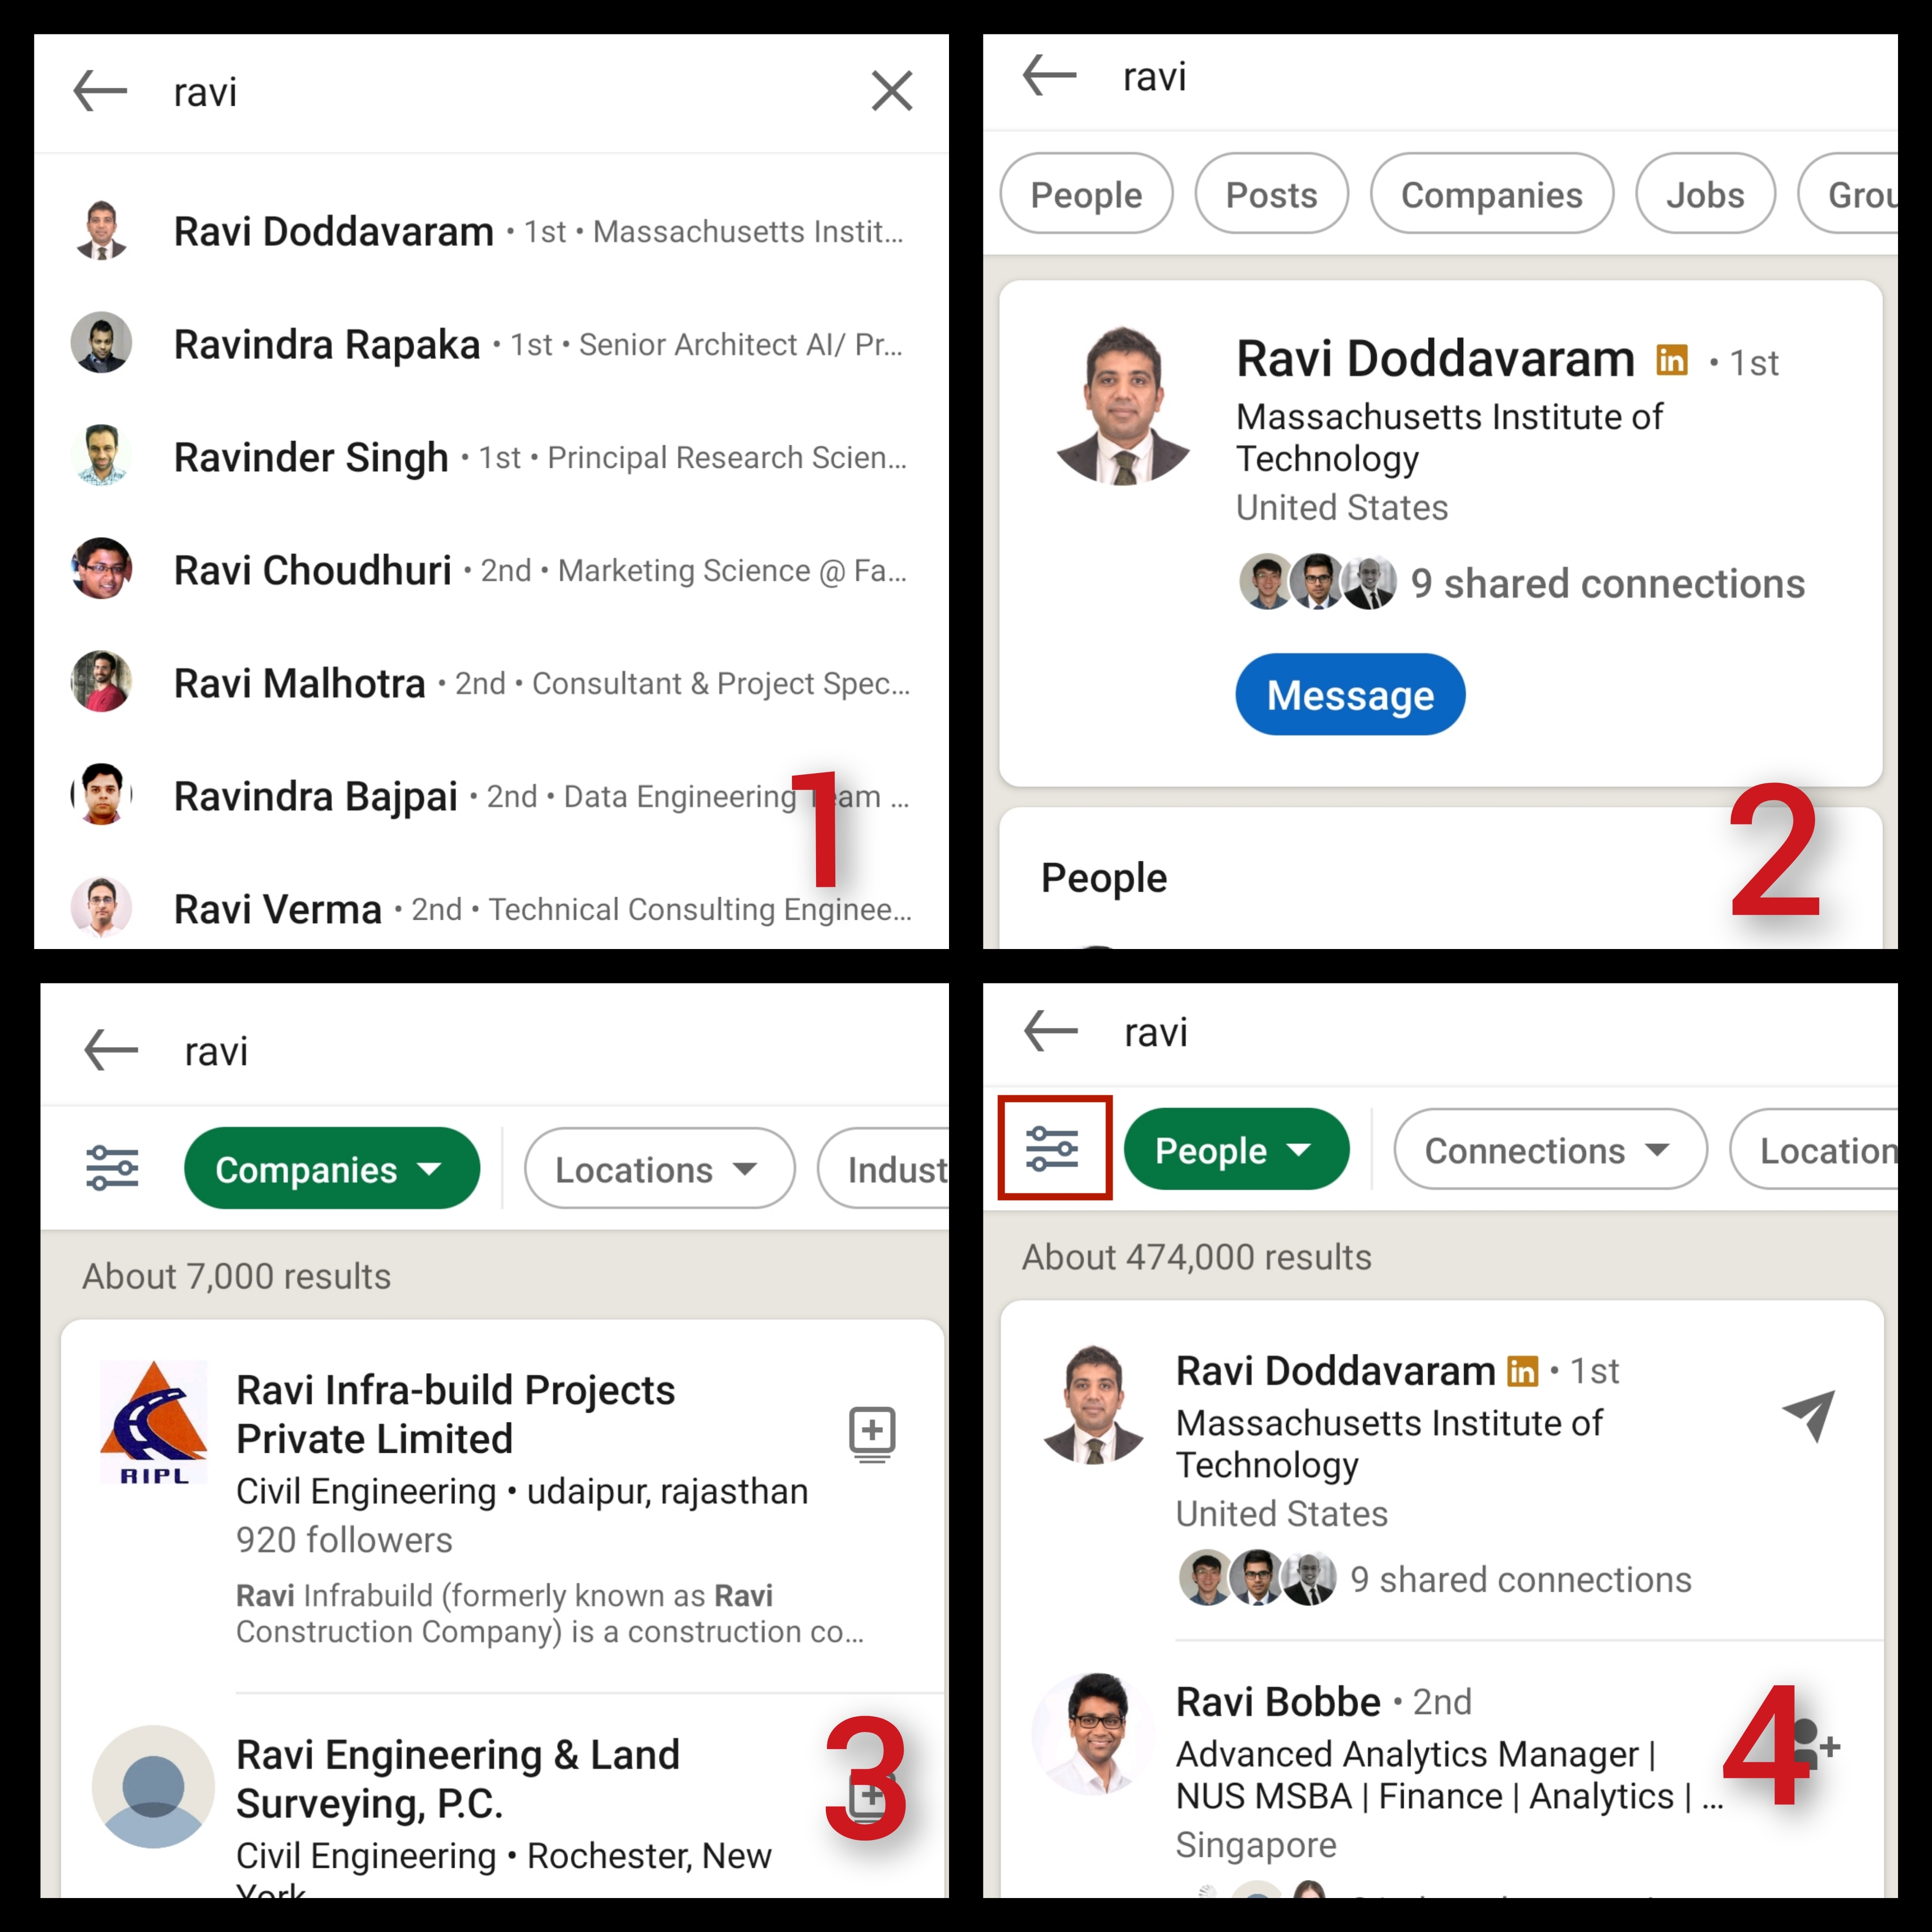
\includegraphics[height=10cm]{jdf-latex/Figures/search_prob.jpeg}
	\caption{1 - searching people's name, 2 - search result page, 3 - click company button, it will show you companies instead of filters 4 - click people button, then use filters on the left to specify a person's company}
	\label{fig:search_prob}
\end{figure}

In 18 out of cases, I can successfully find my target. (18/20 = 90\%) LinkedIn has already done a good job on ranking the search order to help you find the most likely person. But there are mainly 3 issues raised from my search.

First, as shown in Figure 1, I used the LinkedIn mobile app to search for a person's name, then on the result page I would like to further refine my search using company filter. I almost always click the "Companies" button and it is not the filter button I need. 
Second, I need to search both Chinese name and English name, and the combination of the two to find a Chinese co-worker. This is generally the case for those who work in China, Hong Kong or Singapore. LinkedIn is not specialized in dealing with multi-language search.
Third, if a person is not on LinkedIn, which is quite often the case for academics, I would fail the task.

\subsection{Takeaways}
LinkedIn search function is good enough in common cases, though there are some room for improvements for the edge cases like I mentioned above. The search result page can be better designed for tasks under different context.

\subsection{Biases Control}
Participant observation can be biased if you overly represent your own experience. (Joyner, 2021) Through my own observation, I tend to have confirmation biases and ignore the useful information. The problem raised in my own participant experience may not be a general issue for people to accomplish the task. In order to avoid the confirmation biases from this exercise, I will ask the same question during the interview to verify it is a general problem.

\section{Needfinding Execution 2 - Interview}
\subsection{Steps}
10 working adults are interviewed for this LinkedIn searching function task. Because the way LinkedIn designed is for professional connections. 5 questions have been asked during the interview to gather the response of usability of LinkedIn search function.

\subsection{Raw Results}
4 out of 10 find LinkedIn search function easy to use. They are always able to find the person they need. 4 out of 10 find LinkedIn search function hard to use. The results are always not relevant. And 2 out of 10 do not use the search function at all. The normal use cases are to search newly joined colleagues, to search the upcoming interviewers and to search the target customers background. Raw questions are in the appendices.

\subsection{Takeaways}
As Joyner said, "You are not your user!" (Joyner, 2021b). The people I interviewed had many different experience comparing to mine. Through Interview we gathered richer and more holistic data comparing that through participant observation. 

\subsection{Biases Control}
The confirmation biases are avoided here because the conclusion from participant observation are further verified here. One of the interviewees had the same issue, not able to properly use filter in the search result page. An interesting finding is that, despite 4 of them said the search function is easy to use, 3 of them were making the same mistake when asked to use company filter in the people search result page. By doing the task under this context, we avoid the recall biases that people tend to forget the difficulties they met after they finished the task for a while. Also, to avoid social desirability biases, most of the questions are formatted as open-ended questions. To have more confidence in the problems raised in interviews, we can further examine those problems using the survey methods to reach a larger audience base.

\section{Needfinding Execution 3 - Survey}
\subsection{Steps}
In this needfinding execution, 25 people are surveyed for 16 questions about LinkedIn Search Functions. Raw responses and questions in the appendices. Survey was posted in the peersurvey website for HCI course, and it closed after gathered 25 responses.

\subsection{Raw Results}
Raw response can be found in the appendices. We can see that most of the people in the age group 18-39, and most of the people are satisfied with existing search function. More than half of the people are using LinkedIn for finding jobs and about half are using LinkedIn to find people. Most of the people are not frequent users. About 2/3 of the devices are PC and laptops, so the website experience matters more. And people generally have the needs to search for co-workers.

\subsection{Takeaways}
We can see a variety of goals when people are using LinkedIn and what they are searching for. They tend to be OK with the existing search function design. But through the last experiment we can see that, even interviewees OK with the existing design can make the the mistake and fail the task. 

\subsection{Biases Control}
In order to avoid social desirability biases, survey questions are phrased in a neural way. Since in HCI peersurvey website generally people are more willing to help other students to finish the survey, voluntary response bias is avoided. But this survey will certainly suffer from recall biases. For the complex task like using company filter in people search result, we cannot have a good response from survey. We need to gather that type of data through other needfinding methods. Also, this survey suffers from the biases that most of the responses are from OMSCS HCI students. More responses from other channels may be needed.


\section{Data Inventory}
These are the questions we want to answer though our needfinding exercises: (Joyner, 2021a)
\begin{quotation}
	\noindent
	\begin{itemize}
	    \item Who are the users?
	    \item Where are the users?
	    \item What is the context of the task?
	    \item What are their goals?
	    \item What do they need?
	    \item What are their tasks?
	    \item What are their subtasks?
    \end{itemize}
\end{quotation}

Now we will go through each question and see if our needfinding executions have answers.

\subsection{Who are the users}
First type of users are the power users of LinkedIn like myself. I don't have many power users in the interviews or surveys. Second type of users are working adults who occasionally use LinkedIn, which are the most of my interviewees and survey participants.

\subsection{Where are the users}
Since this is a website or an mobile app, people are either using phone, laptop or PC in the workplace to access LinkedIn. There are scenarios when people using LinkedIn app in other places, but chances are those would still be some professional occasions. In the survey questions, we can see most of the people are using desktop or laptop, meaning most of the time it is used in workplace or professional occasion.

\subsection{What is the context of the task}
From the above finding, we understand that most of the time people using LinkedIn in workplace, so their priority would still be the daily work. The users will be distracted, so the process is better to be easy, fast and accurate. 

\subsection{What are their goals}
Through the survey we can see the the appendices that, most of the goals are finding jobs and find people they know. Also, near half of the people would like to search about companies as well. Their goal is to have the correct result in the search result page. We can see from the survey that most of the time people are not using it for searching posts.

\subsection{What do they need}
What they need in this task is normally the names of the person or company. But it can be challenging when it involves multi-languages. One thing missed in my survey is people with multi-language needs, since majority of the responses come from US. If the name is too common, people need to add filters to refine the search. This data is gathered through participant observation and interviews, and it can hardly be addressed through surveys. The data needs to be collected through the process of performing the task.

\subsection{What are their tasks}
The tasks are tightly connected with the goals. To search a person, one needs to key in the person's name to search, same for searching companies. Searching jobs is a bit different, you need to provide both the name of the job and a location. For all three goals, the tasks are relatively the same - key in the names and find the results in the search result page. There are multiple other tasks they can perform in the LinkedIn interface, and there are other distractions in the workplace environment. A good design should be capable to let the user accomplish the task given those contexts.

\subsection{What are their subtasks}
The data for collection subtasks are mainly from participant observation. The needfinding methods that can help with subtasks inventories are participant observation, ethnography and naturalistic observation. It is not feasible to do naturalistic observation for the task using LinkedIn application. And ethnography may be suitable for more complex task like video editing. Through participant observation, I found the issue on one of the subtasks - the filter in search result page is hard to use. Also, from the interviews, we understood that often the search result it not relevant. The cluttered result interface contains people, companies, and posts results. It violates the tip that "Emphasizing essential content while minimizing clutter" (Joyner, 2021d) as well. But the issue of collecting subtasks through participant observation only is that it overly represents my own experience. In the next iteration of needfinding, I need to examine the subtasks by observing other participants doing the same tasks.

\section{Defining Requirements}
Based on the result of our needfinding exercises, we can define the requirements for our interface. It turns out most of the users are novice users (less frequent users), the interface should be guide the user though the task. But also people in workplace have limited resource and time in this task, so efficiency is as important as learnability. Also, since people are using the interface both on mobile and desktop/laptop, the interface should be catered for both app and website. All requirements are summarized in below Table 1.

\begin{table}[h] % [h] forces the table to be output where it is defined in the code (it suppresses floating)
	\caption{Requirements from Needfinding}
	\small % Reduce font size
	\centering % Centre the table
	\begin{tabular}{L{0.13\linewidth} L{0.13\linewidth} L{0.13\linewidth} L{0.13\linewidth} L{0.13\linewidth} L{0.13\linewidth}}
		\textbf{\-} & \textbf{Functionality} & \textbf{Usability} & \textbf{Learnability} & \textbf{Compatibility} & \textbf{Efficiency}\\
		\toprule[0.5pt]
		\textbf{Requirements} & User can find target in the search result & It is easy for the user to search & It takes little time for user to learn interface & The interface works on both mobile and website & The interface can also help expert user to accomplish task efficiently \\
		\midrule
		\textbf{Evaluation} & How many times user can find target in result & Interface is rated as easy to use for most users & How fast user start to use the interface & Users can accomplish task on both mobile and website & Users can finish task faster with shortcuts \\
	\end{tabular}
\end{table}

\section{Continued Needfinding}

Through this needfinding exercise I found the needfinding exercise is very likely to be an iterative progress. We do not know much about our users in first place. Multiple needfinding methods work together can give us a more holistic view about the task and the context of the task. 

\begin{quotation}
"What remaining questions are there that would benefit from additional needfinding investigation?"
\end{quotation}

As mentioned in section 4.7, conclusions from participant observation need to be further verified through other needfinging methods like interviews or surveys. Also, we do not have enough data inventory for the task that people are searching jobs instead of people. We can have more questions to understand that task.

\begin{quotation}
"What new questions arose during this initial round of needfinding?"
\end{quotation}

Problems raised from interviews can be formatted as survey questions, then we can refine our survey to have better understanding about whether the problem of the interface is really affecting people to accomplish the task. Also, we will ask more questions about problems when people using LinkedIn search function to find jobs or companies.

\begin{quotation}
"What types of exercises would you do next to address these remaining or new questions?"
\end{quotation}

All three needfinding exercises will be done with new questions. Through participant observation we can find subtasks and issues for the companies and jobs searching task. New questions in survey and interviews can further verify the issues in these 2 tasks and refine the needs when people are using LinkedIn search function.

\section{References}

[1] Joyner, D. (2021a). Data Inventory. Udacity.

https://classroom.udacity.com/courses/ud400/lessons/9662642568/

concepts/96550826820923

[2] Joyner, D. (2021b). 5 Tips: Interviews. Udacity. 

https://classroom.udacity.com/courses/ud400/lessons/9662642568/

concepts/97510951660923

[3] Joyner, D. (2021c). Defining the Requirements. Udacity. 

https://classroom.udacity.com/courses/ud400/lessons/9662642568/

concepts/96759245540923

[4] Joyner, D. (2021d).5Tips: Reducing Cognitive Load. Udacity. 

https://classroom.udacity.com/courses/ud400/lessons/9232968306/

concepts/92293480800923

\section{Appendices}

\subsection{Interview Questions}

\begin{enumerate}
    \item Do you use LinkedIn search function?
    \item Under which scenarios you are using LinkedIn Search function?
    \item Do you think LinkedIn search function is easy to use?
    \item What do you think LinkedIn search function can be improved?
    \item How much do you satisfy with current LinkedIn search function?
\end{enumerate}  

\subsection{Survey Raw Data}
\begin{figure}[h]
	\centering
	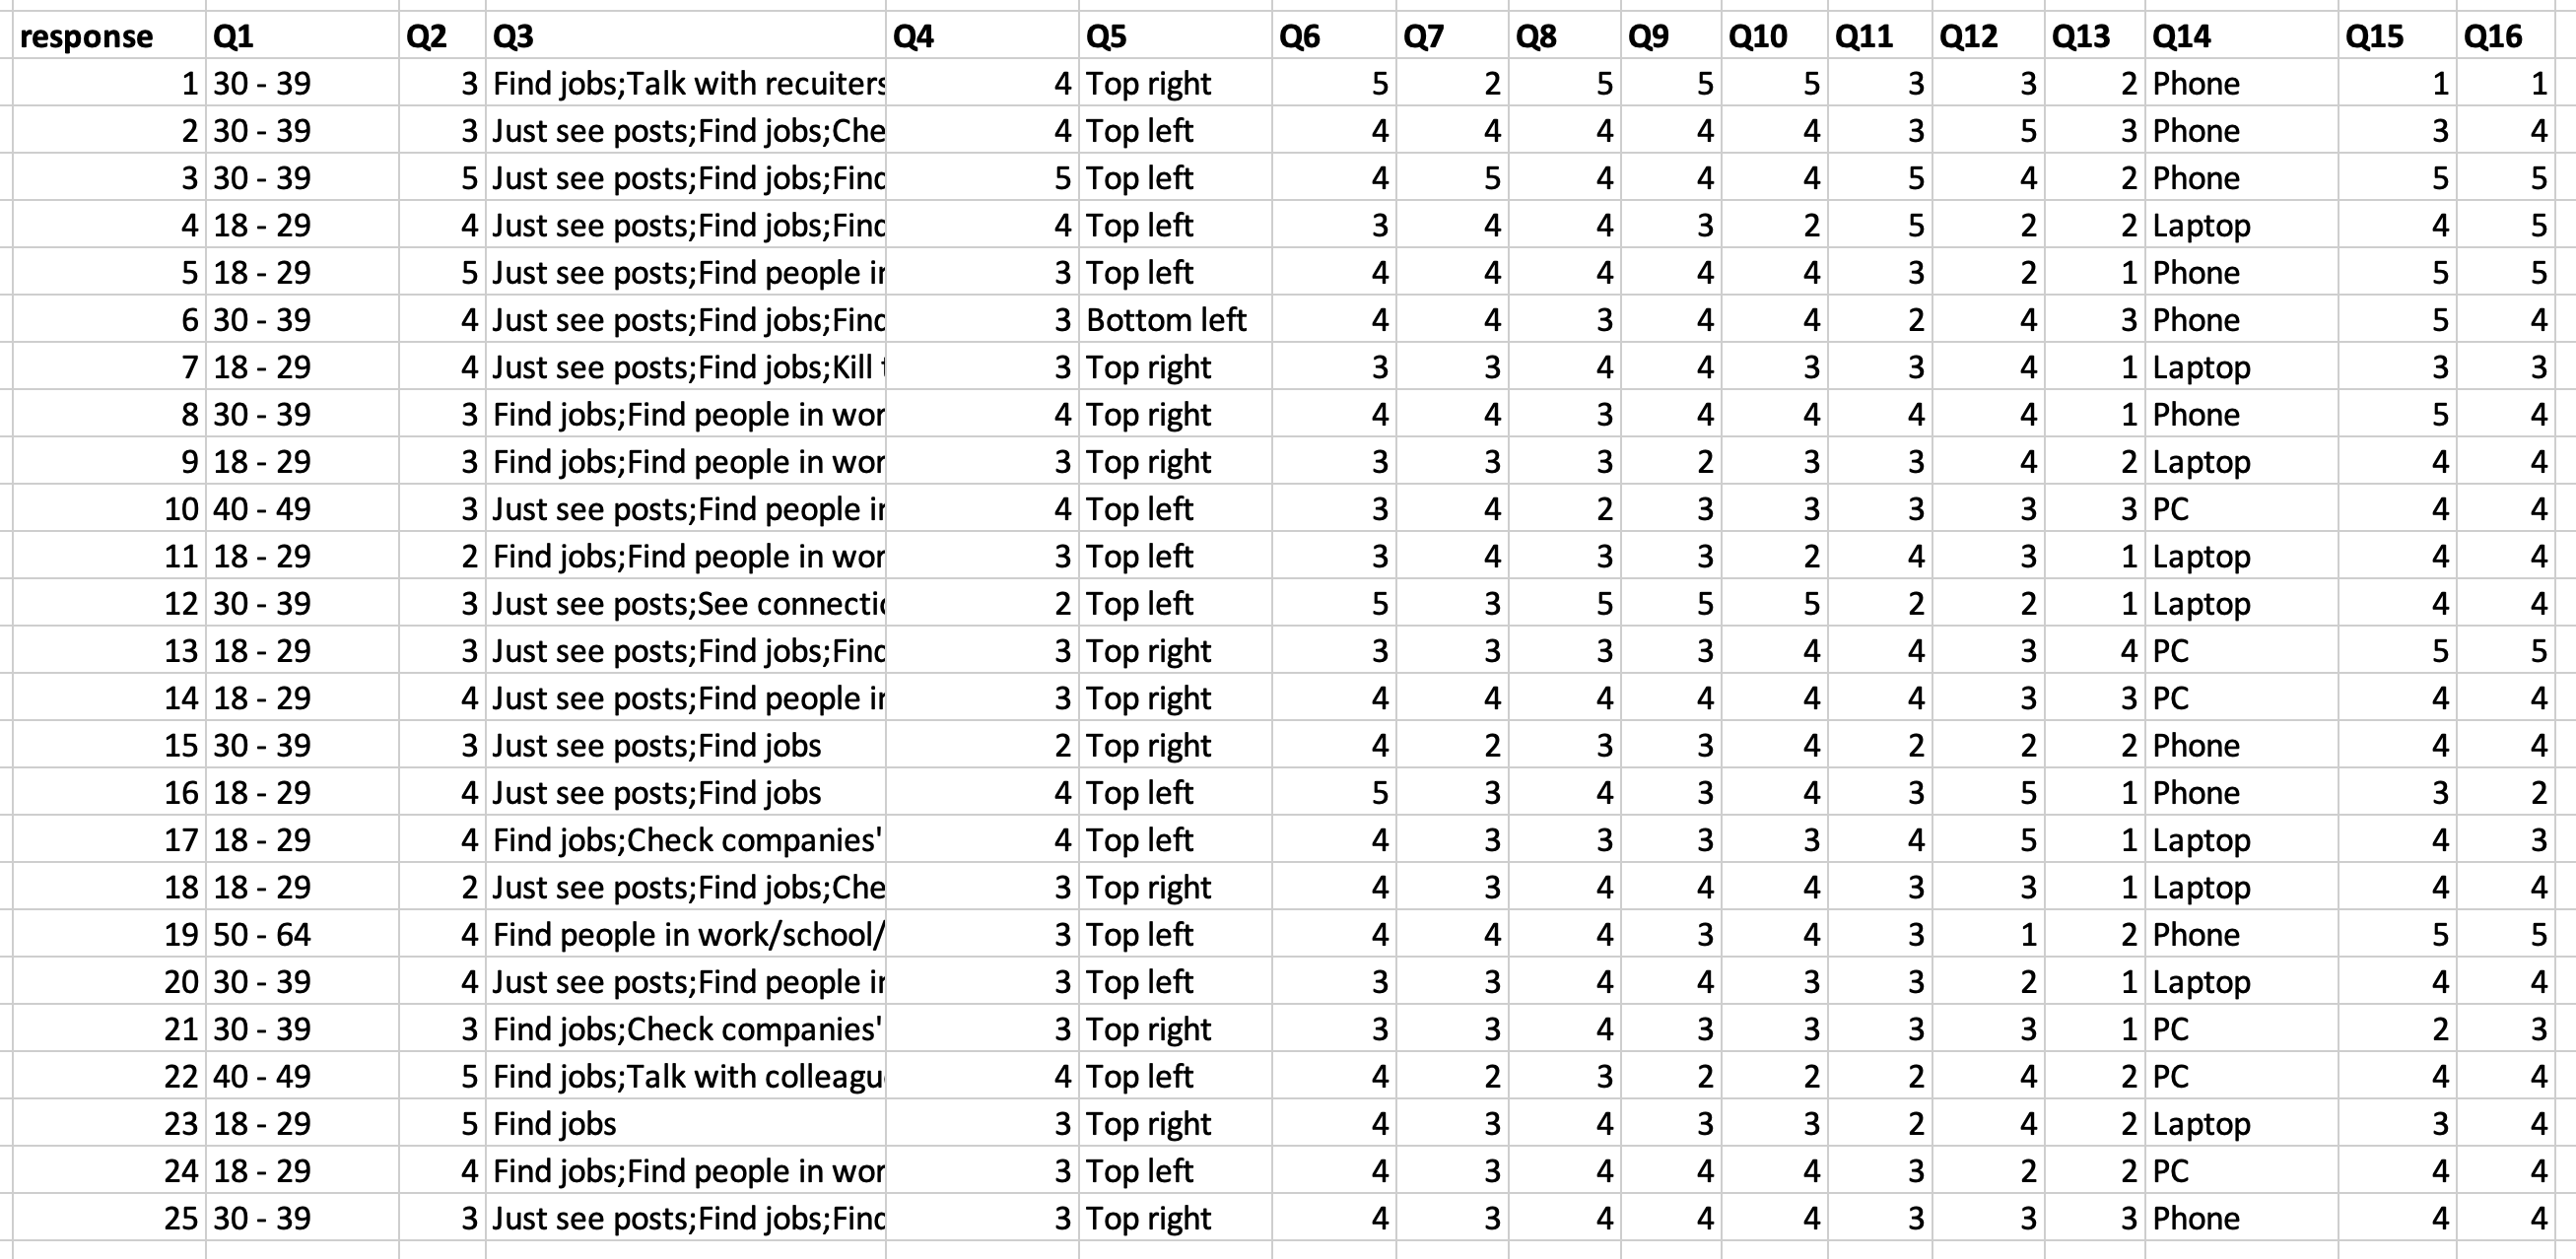
\includegraphics[height=10cm]{jdf-latex/Figures/survey_raw.png}
	\caption{Raw data from Survey}
	\label{fig:survey_raw}
\end{figure}

\begin{figure}[h]
	\centering
	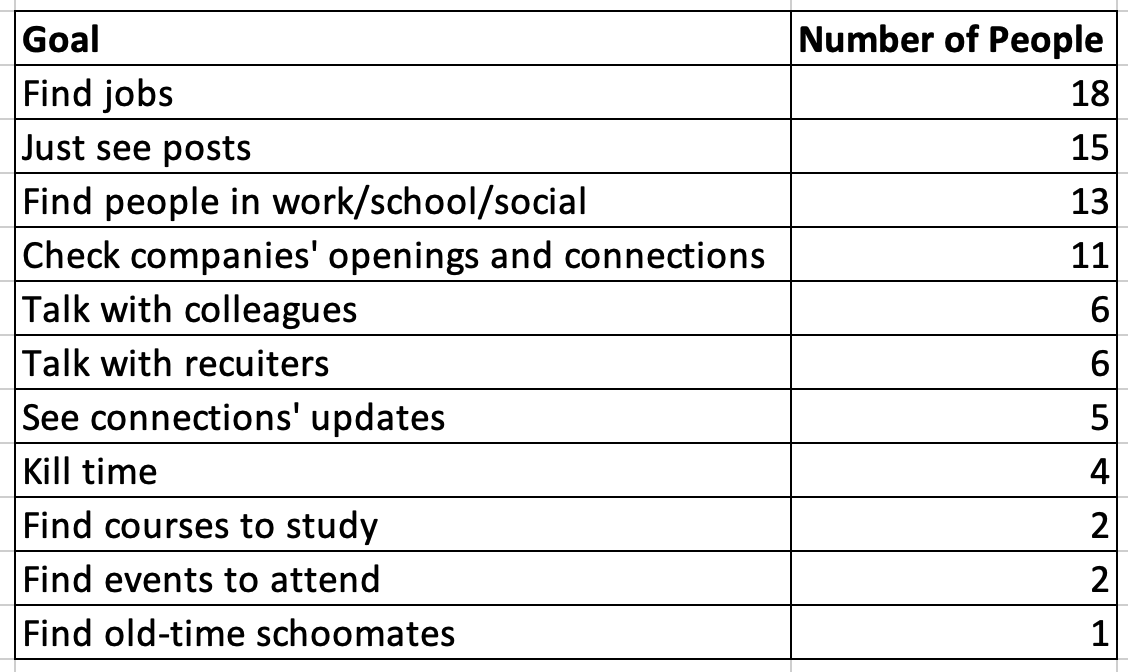
\includegraphics[height=6cm]{jdf-latex/Figures/search_goals.png}
	\caption{Why people using LinkedIn Search Function}
	\label{fig:search_goals}
\end{figure}


\subsection{Survey Questions}
\begin{enumerate}
    \item Select your age
    \item How often do you use LinkedIn
    \item What do you mostly do with LinkedIn
    \item How often do you use LinkedIn Search box
    \item Where would you prefer to see the Search box on the screen
    \item It is easy to use the current LinkedIn Search Box
    \item How often do you use Search Box to find people
    \item It is very easy for me to search for people on LinkedIn
    \item It is easy to filter the people search results
    \item It is easy for me to search for people using LinkedIn mobile app
    \item How often do you use Search Box to find companies
    \item How often do you use Search box to find jobs
    \item How often do you use Search box to find posts
    \item Which is the device you are mostly using LinkedIn app on
    \item I would like to check my colleague's background on LinkedIn
    \item I would like to know the event speaker's background on LinkedIn
\end{enumerate}

\end{document}